\documentclass[reprint]{revtex4-1}

\usepackage{xparse}
\usepackage{xfrac}
\usepackage{graphicx}
\usepackage{mathtools}

\usepackage{paralist}

\usepackage{subcaption}
\usepackage{threeparttable}
\usepackage{multirow}

\usepackage{url}
%\usepackage{hyperref}

\DeclareDocumentCommand{\CS}{sO{}}{\IfBooleanTF{#1}{\hat{\sigma}_{#2}}{\sigma_{#2}}}
\DeclareDocumentCommand{\slp}{sO{}}{\IfBooleanTF{#1}{\hat{\beta}_{#2}}{\beta_{#2}}}
\DeclareDocumentCommand{\Thick}{O{}}{\Theta_{#1}}

\DeclareDocumentCommand{\SE}{sm}{\IfBooleanTF{#1}{\hat{\sigma}\bkt*{#2}}{\sigma\bkt*{#2}}}

\DeclareDocumentCommand{\bkt}{sm}{\IfBooleanTF{#1}{\left[ #2 \right]}{\left(#2\right)}}
\newcommand{\td}{\mathrm{d}}

\DeclareDocumentCommand{\ADCcode}{O{ }}{unit{#1}}

\newcommand{\scl}{.4}

\DeclareDocumentCommand{\Ayy}{s}{\IfBooleanT{#1}{\hat}A_{y,y}}


\begin{document}
\begin{abstractname}
We summarize a procedure of estimating unpolarized $pp$ cross section from beam current data in a transmission experiment. The methodology presented is grounded in the use of the optical theorem.
\end{abstractname}

\section{TRIC program}

TRIC (test of Time-Reversal Invariance at COSY) is a transmission experiment planned at the cooler synchrotron COSY-Juelich for the purpose of testing Time-Reversal Invariance. Its physical foundation is the use of a genuine null-observale for T-symmetry, --- the total cross section asymmetry in double-polarized proton-deuteron scattering, --- whoose existence is guaranteed by the optical theorem.~\cite{Conzett} TRIC is aimed at achieving the accuracy of $10^{-6}$ in the cross section asymmetry estimate.

The total cross section in a double-polarized scattering involves a number of polarization-dependent terms:
\[
	\CS[tot] = \CS[0]\cdot\bkt{1 + \sum_{i,j} A_{i,j} P_iP^t_j},
\]
where $P^t_j$ and $P_i$ are respectively the $j$-projection of target and $i$-projection of beam polarizations, $\CS[0]$ is the unpolarized cross section component, and $A_{i,j}$ is the appropriate asymmetry.

The asymmetry that serves as the null-observable of T-symmetry is $A_{y,xz}$, all others being faking observables. TRIC's experimental design limits the influence of all faking observables to below the experimental accuracy; except for that of $A_{y,y}$, caused by the misalignment of the target and beam polarizations.~\cite[p. 11]{Proposal} Thus arises the problem of knowing the extent to which vector target polarization must be controlled, for which the knowledge of the value of $A_{y,y}$ is required. 

Unpolarized cross section is a parameter in both estimators' distributions, and hence it must be known as well. 

\section{Theory}
\subsection{Physics}
The intensity of a particle beam revolving inside an accelerator decreases according to the Beer-Lambert law:
\begin{align*}
	I_{n+1} &= I_n \cdot \exp\bkt{-\sum_{i=i}^N \CS[i]\cdot\int_0^L n_i(z)\td z} \\
			&= I_n \cdot \exp\bkt{-\sum_{i=i}^N \CS[i]\cdot \Thick[i]} \\
			&= I_n \cdot \exp\bkt{-\sum_i\frac1\tau_i},
\end{align*}
where $L$ is the beam path length, $N$ is the number of attenuating species, $\CS[i]$ is the attenuation cross section, $n$ is the number of passed revolutions, $\Thick[i] = \int_L n_i(z)\td z$ is the thickness of the corresponding attenuating species.

For the average beam current, integration of the above yields
\begin{equation}\label{eq:CurrentDecay}
	I_t = I_0 \cdot \exp\bkt{\slp\cdot t},
\end{equation}
with $\slp = \sum_i \slp[i] = - \nu\cdot\sum_i \sfrac1\tau_i$, $\nu$ --- the beam revolution frequency. 

Within the confines of the experiment, an unpolarized proton beam interacts with an unpolarized deuterium target with cross section $\CS[0]$; to that add all extra-target losses ($\CS[x]\Thick[x]$), to produce the following expression for beam loss:
\begin{equation}\label{eq:SlopeModel}
	\slp = -\nu\bkt{\CS[0]\Thick + \CS[x]\Thick[x]}.
\end{equation}

Since $\CS[x]\Thick[x]$ is independent from the target state, an estimate of the cross section is obtained from  
\begin{equation}
	\CS*[0] = \frac{\slp*[off] - \slp*[on]}{\nu\Thick[on]},
\end{equation}
where $\slp*[on/off]$ is the slope estimate in an on-/off-cycle.

The expression for the polarized beam loss is 
\[
	\slp = -\nu\bkt{\CS[0](1 + \Ayy P_y^t P_y)\Thick[on] + \CS[x]\Thick[x]},
\]
from which an asymmetry estimate can be computed as the difference between the slopes with spin states \emph{up} and \emph{down}:
\[
	\Ayy* = \frac{\slp*[on]^- - \slp*[on]^+}{\nu P_y^t\Delta P_y\cdot \CS[0]\Thick[on]}.
\]

\subsection{Statistics}

We estimate $\slp$ by fitting a linear model to logarithmized beam current data, $\ln I_t = \ln I_0 + \slp\cdot t + \epsilon_t$, using the least squares method. In order that the estimate be minimum-variance mean-unbiased, the data must satisfy the Gauss-Markov conditions:~\cite{GaussMarkov}
\begin{enumerate}
	\item Linearity and additivity of the relationship;
	\item Independence of the time and error variables (strict exogeneity);
	\item No serial correlation of the error;
	\item Constant variance of the error (homoskedasticity).
\end{enumerate}

Linearity is necessary for the validity of using linear regression; homoskedasticity and absence of serial correlation are required for the efficiency, and exogeneity for the consistency of the estimator.

This means the following series of questions has to be answered in order to verify the validity of our results:
\begin{enumerate}
	\item Is the logarithm of beam current a linear function of time?
	\item Are the errors uncorrelated with time?
		\begin{itemize}
			\item Is measurement time measured with negligible error?
			\item Are there predictors other than time?
			\item Is there among the omitted variables a predictor dependent on current?
		\end{itemize}
	\item What is the interpretation of the slope?
\end{enumerate}

Below, we will be concerned with the former two.

\section{Overview of data}
We have analyzed two data sets: one was measured in 2012, the other in 2016. 

In the 2012 experiment, the beam and the target both consisted of unpolarized protons; the beam was cooled using electron cooling and bunched by the barrier bucket; the cycles lasted for one hour each. In the 2016 experiment the proton beam was scattered on the deuteron target, both polarized; the beam had undergone RF-bunching and electron-cooling; the cycles lasted for 12 minutes, the first half of which the target was turned on, in the second off; the beam spin state alternated from spin up to spin down through no spin, while the target spin state remained constant (spin up). 

\begin{figure}[h]
\begin{subfigure}{.5\textwidth}
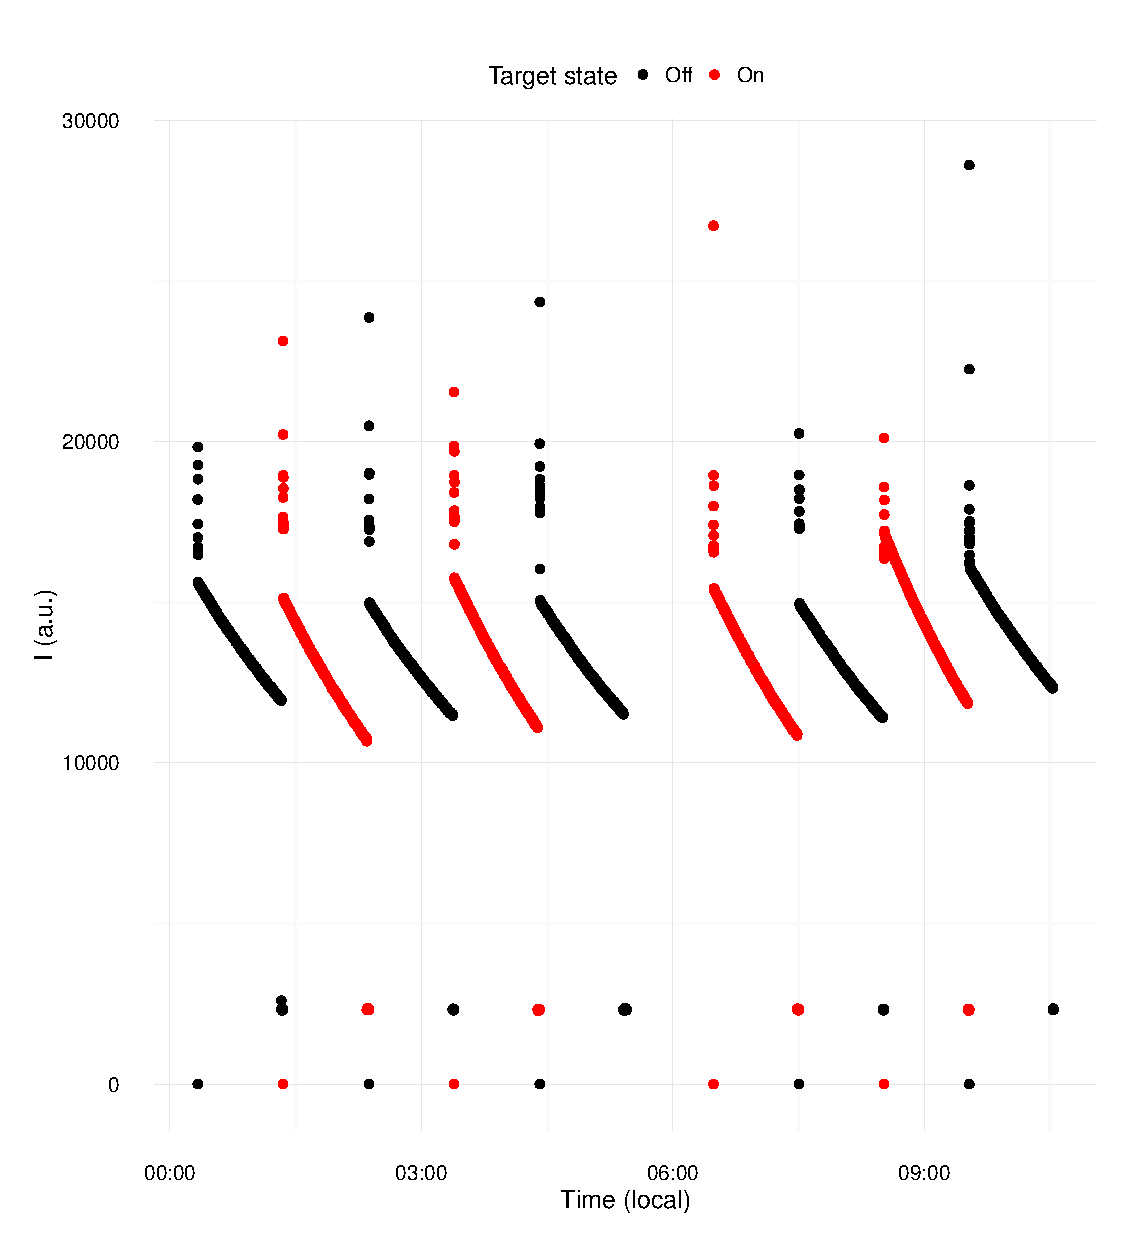
\includegraphics[scale=\scl]{img/Cycles2012.eps}
\caption{Experiment in 2012. The cycles with the target are drawn in red, those without in black. \label{fig:Cycs2012}}
\end{subfigure}
\begin{subfigure}{.5\textwidth}
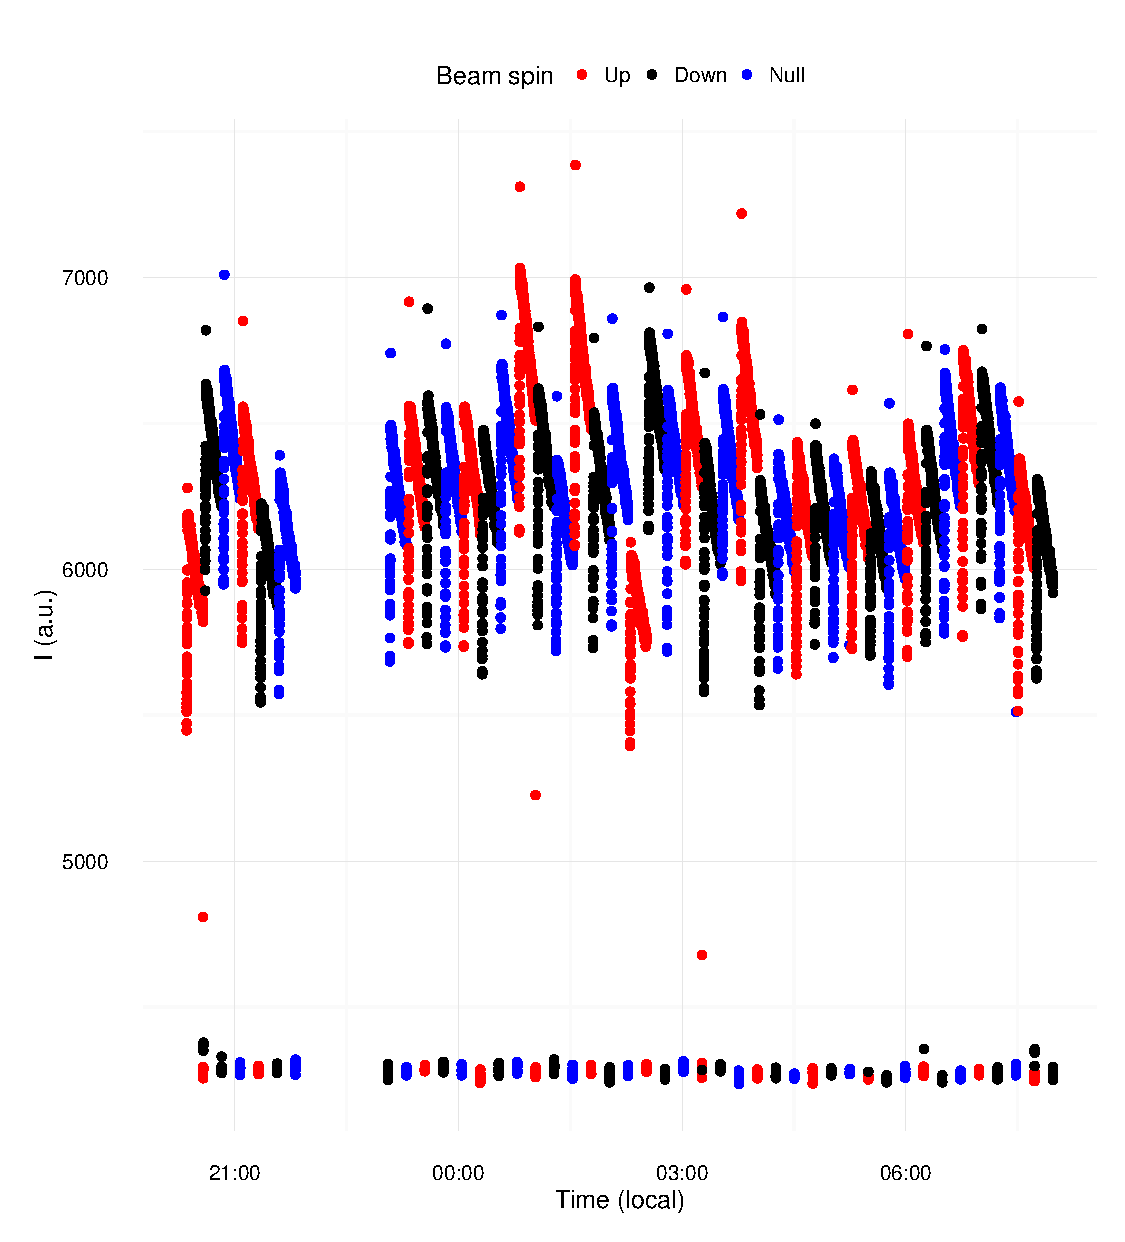
\includegraphics[scale=\scl]{img/Cycles2016.eps}
\caption{Experiment in 2016. The cycles are colored according to the beam spin state.\label{fig:Cycs2016}}
\end{subfigure} 
\caption{Average beam current as a function of time.}
\end{figure} 


\section{Estimation of slope}

In order to correctly estimate a cycle's slope, we subtract the BCT offset $\Delta$ from the data. This is done  because
\begin{align*}
	\tilde{\slp} &= \frac{\td\ln \tilde{I}_t}{\td t} 
				  = \frac{1}{\tilde{I}_t}\frac{\td \tilde{I}_t}{\td t}, 
\shortintertext{where, if the measured current}
	\tilde{I}_t  	&= I_t + \Delta_t = I_0\exp\bkt{\slp\cdot t} + \Delta_t, 
\shortintertext{then}
\tilde{\slp} 	&= \frac{1}{1 + \lambda_t}\bkt{\slp + \frac1{I_t}\frac{\td\Delta_t}{\td t}}, \\
	\lambda_t	&= {I_0}^{-1}\cdot \Delta_t\cdot\exp\bkt{-\slp\cdot t}.
\end{align*}

Even a constant offset must be removed in order to have a constant slope to estimate. The presence of an offset (let alone a time-dependent one) violates the exogeneity assumption, and hence biases the estimate. At this stage, estimation was done assuming offset was constant within a cycle, and its value was estimated as the median of the post-cycle current.

\begin{table}
\centering
\begin{threeparttable}
	\caption{Characteristics of a typical cycle.\label{tbl:CycleChars}}
	\begin{tabular}{llr}
	\hline\hline
	Charactetistic	& Test 					& P-value\\
	\hline
	Linearity 		& Harvey-Collier		& 0\% \\
	-				& Rainbow				& 0\% \\
	Constant slope	& Chow\tnote{a}		 	& 100\% \\
	-				& Moving estimates		& 1\% \\
	Homoskedasticity& Breusch-Pagan 		& 0\% \\
	Autocorrelation & Durbin-Watson			& 0\% \\
	\hline\hline
	\end{tabular}
	\begin{tablenotes}
		\item[a]{The Chow test was performed at every point in the fitting range. The average of F-statistics is used as the test statistic.}
	\end{tablenotes}
\end{threeparttable}
\end{table}

After subtracting the offset, the linear model $\ln I_t = \ln I_0 + \slp t +\epsilon_t$ is fitted via the ordinary least squares method. The reduced chi-squares camputed from model residuals deviate from one starting from the fourth decimal place; however, one should note that the data do not pass linearity tests, and are likely to have structural slope changes as well (see TABLE~\ref{tbl:CycleChars}). Because the model residuals exhibit serial correlation (FIG.~\ref{fig:Run969}), the slope estimates' standard errors are estimated with robust estimators.

\begin{figure}
\centering
\begin{subfigure}{.5\textwidth}
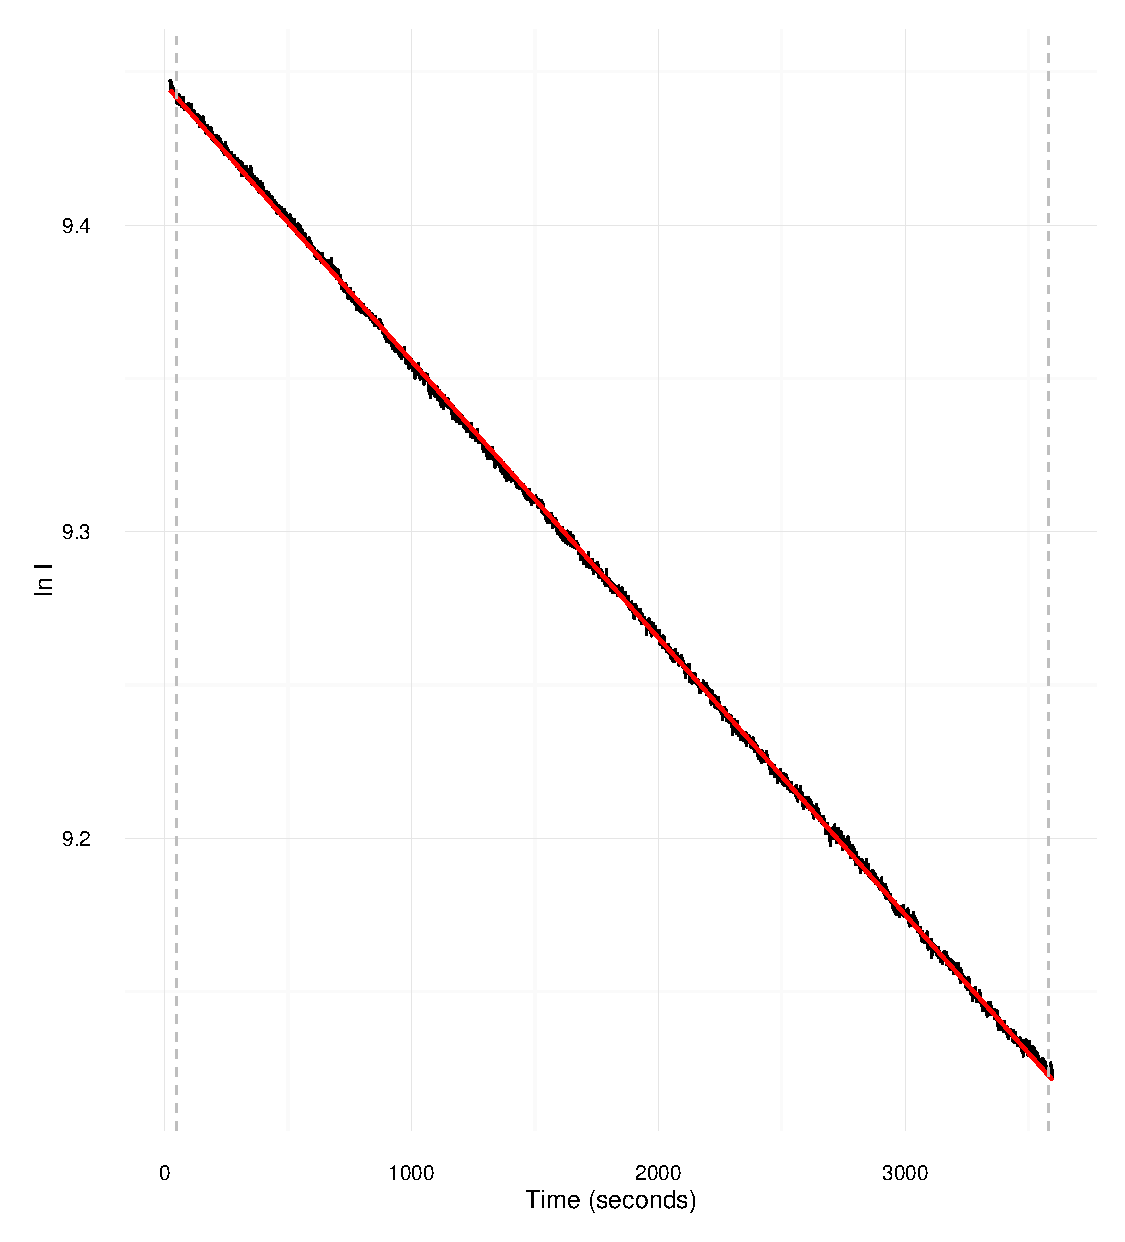
\includegraphics[scale=\scl]{img/Run969_Data_AND_Fit.eps}
\caption{Logarithm of measurement data as a function of time. The fitted line is colored red, the gray dashed lines mark the fit region.}
\end{subfigure}
\begin{subfigure}{.5\textwidth}
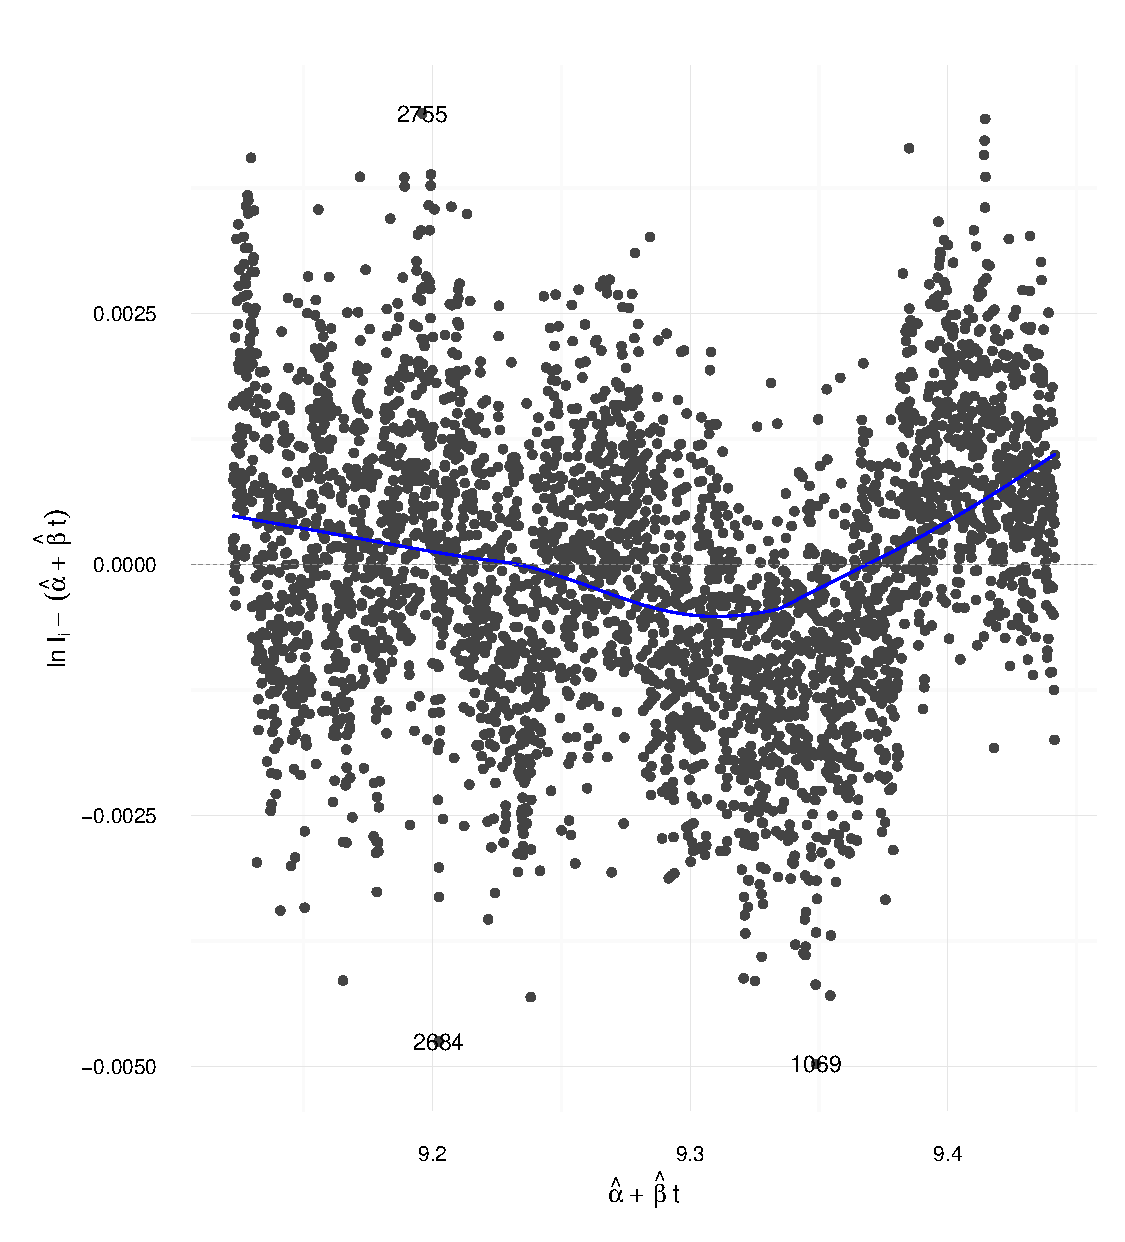
\includegraphics[scale=\scl]{img/Run969_Res_VS_Fit.eps}
\caption{Residuals vs fitted values.}
\end{subfigure}
\begin{subfigure}{.5\textwidth}
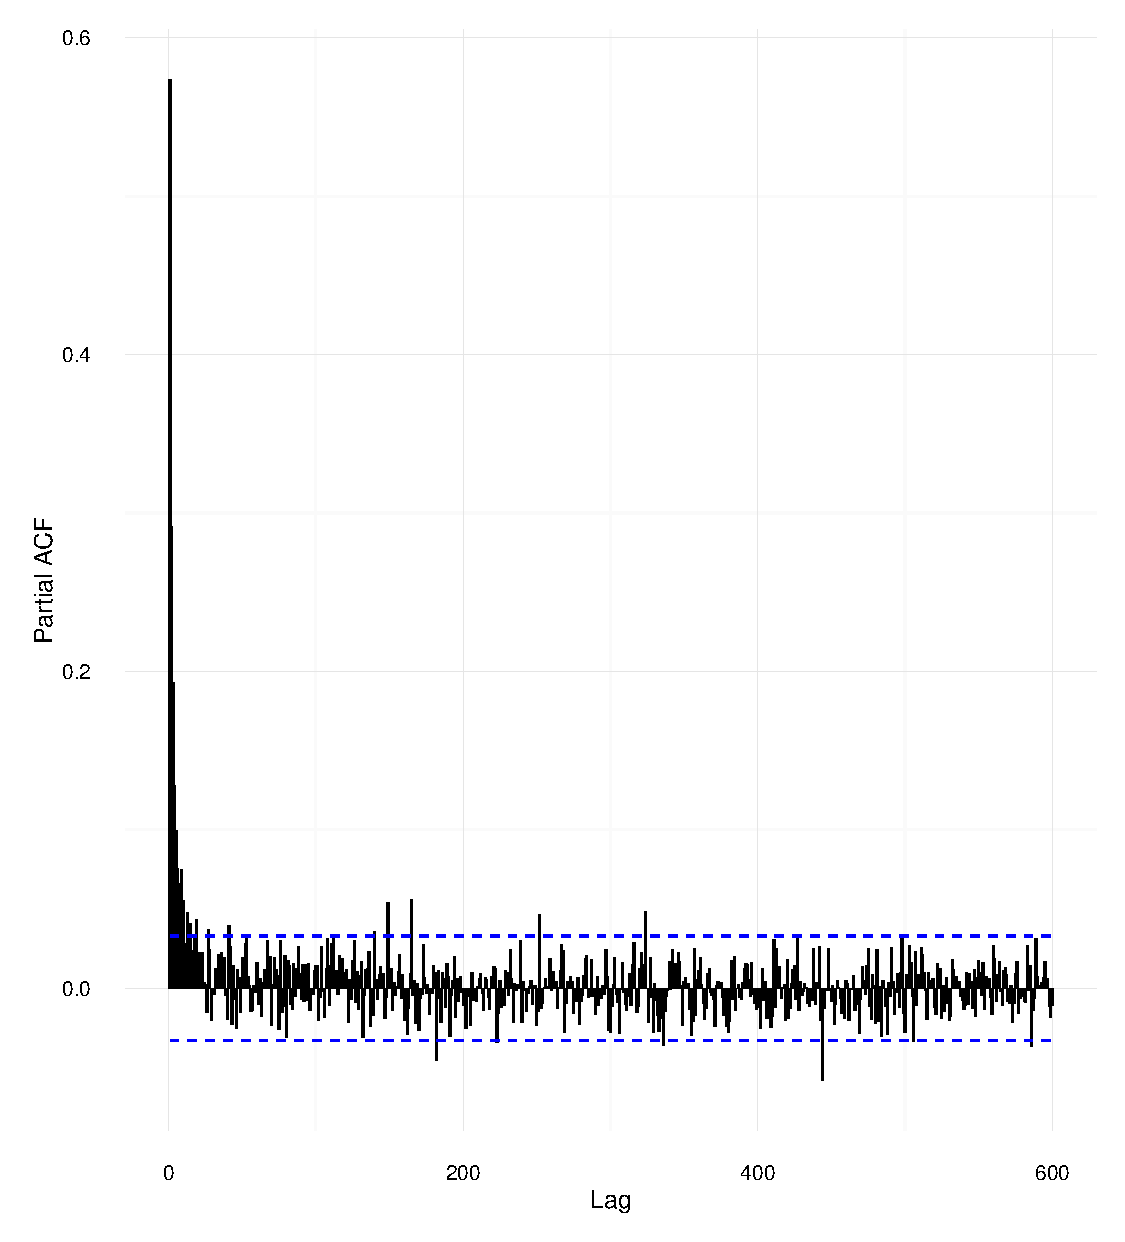
\includegraphics[scale=\scl]{img/Run969_residual_PACF.eps}
\caption{The partial Auto-Correlation Function of the residuals.}
\end{subfigure}
\caption{Some diagnostic plots for a typical cycle.\label{fig:Run969}}
\end{figure}

\section{Estimation of cross section}

In estimating the cross section, we used only the estimates from adjacent cycles. This was done to minimize the effect of drifts of environmental variables such as target thickness, which is estimated to increase by $0.5~ \sfrac{\%}{\mathrm{hour}}$. (The thickness by which the slope differences are divided, assumed constant, was provided by a Schottky measurement.) This reduces the number of estimates from 20 to seven. 

In FIG.~\ref{fig:SlpOnI02016} we plotted the dependence of the slope estimate on the initial beam current, which was estimated by exponentiating the intercept of the fitted model. (If the initial current is also estimated as the median value of current within the second cycle minute, the two estimators are essentially perfectly correlated.) The figure suggests there might be dependence of the estimated slope on the initial beam current; and indeed, when the estimates are fitted with time and initial current used as predictors, the t-test for equality to zero for the beam slope yields p-values less that 1\% for the up and null states, and 5\% for the down state, whereas the time slope's p-value is over 10\% in all cases. The dependency in current is twice as pronounced in the null state, as in the up and down states.

This suggests that to estimate the cross section, one must first adjust the slopes to the same initial current. We do the adjustment as follows:
\[
	\slp*' = \slp* + \gamma(\tilde I_0 - I_0),
\]
where $I_0$ is the initial beam current of the relevant cycle, $\tilde I_0$ is some arbitratily chosen current common for all cycles (we take the median initial current), and $\gamma$ is the slope from the model
\[
	\slp* = \slp*[0] + \gamma I_0.
\]

\begin{figure}
\begin{subfigure}{.5\textwidth}
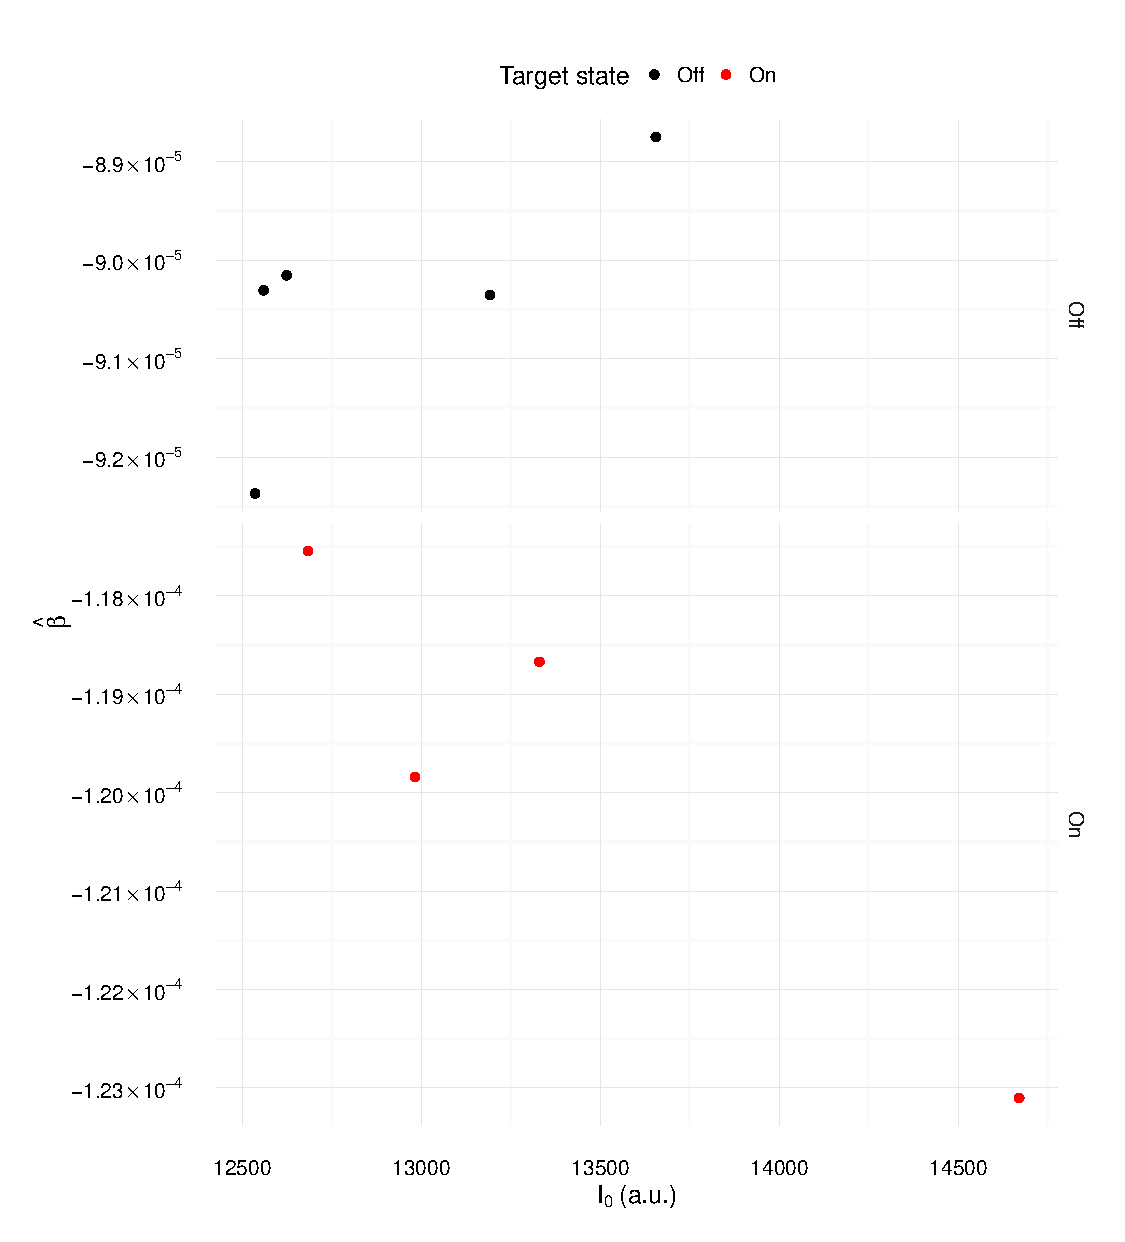
\includegraphics[scale=\scl]{img/Slope_VS_IniCurrent.eps}
\caption{Year 2012.}
\end{subfigure}
\begin{subfigure}{.5\textwidth}
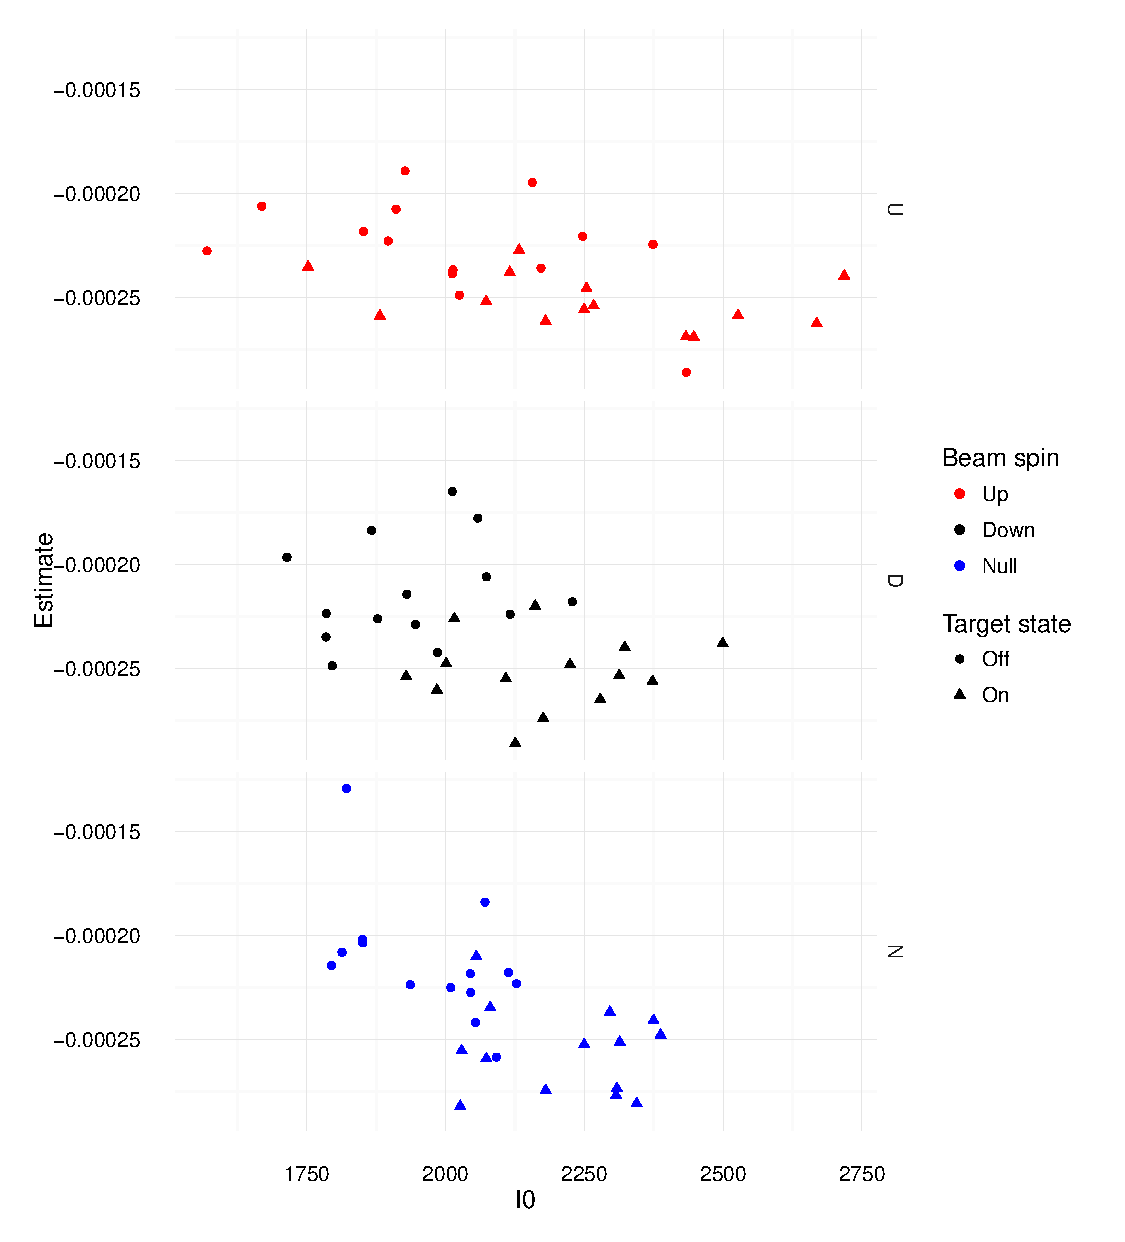
\includegraphics[scale=\scl]{img/Slope_VS_IniCurrent_2016.eps}
\caption{Year 2016.\label{fig:SlpOnI02016}}
\end{subfigure}
\caption{Slope estimates plotted against initial beam current estimated as the exponentiated intercept of the fitted model.}
\end{figure}

An estimate of a cross section estimate's standard error (SE) is made by adding the squared standard errors of the paired slopes, not taking account of the covariance term:
\begin{equation}
	\SE*{\CS*[0]} = \sqrt{\SE*{\slp*[off]}^2 + \SE*{\slp*[on]}^2}.
\end{equation}

This is done so because depending on whether an on-slope is paired with the preceding or succeding off-slope, the covariance term changes sign. Since there's no criterion favoring either of the two mappings, the covariance term was omitted.

\section{Estimation of asymmetry}

\pagebreak

\section{Results}
\begin{table}
\centering
\begin{threeparttable}
\caption{Cross section summary statistics. \label{tbl:CS-all}}
\begin{tabular}{c|llrcr}
\hline\hline
Year						& Soundness		& Closeness		& \#		& Mean\tnote{a} (a.u.)	& SE (a.u.) \\
\hline
\multirow{4}{*}{2012}		& Sound			& Close			& 4			& 507(507)				& 7  \\
							& Sound			& Far			& 8			& 553(563)				& 14 \\
							& Unsound		& Close			& 3			& 562(580)				& 36 \\
							& Unsound		& Far			& 5			& 515(512)				& 20 \\
							& All			& 				& 20		& 536(544)				& 10 \\
\hline					
\multirow{4}{*}{2016}		& Sound			& Close			& 40		& 409(411)				& 48 \\
							& Sound			& Far			& 92		& 396(385)				& 34 \\
							& Unsound		& Close			& 4			& 1400(1418)			& 170\\
							& Unsound		& Far			& 8			& 1453(1457)			& 69 \\
							& All			& 				& 144		& 486(473)				& 35 \\
\hline\hline
\end{tabular}
\begin{tablenotes}
\item[a] The value in parenteses is the weighted mean with measurements' variance estimates used as weights.
\end{tablenotes}
\end{threeparttable}
\end{table}

The summary statistics of cross section estimates, grouped by soundness and closeness of the slope estimates they are based on, are presented in TABLE~\ref{tbl:CS-all} and FIG.~\ref{fig:CS-all}; the slopes themselves are shown in FIG.~\ref{fig:Slopes} and summarized in TABLE~\ref{tbl:Slp-big}. Group density estimates with the rectangular kernel are shown in FIG.~\ref{fig:CS-dens}.

\begin{table}
\centering
\caption{Slope summary statistics. \label{tbl:Slp-big}}
\begin{tabular}{llrr}
\hline\hline
Target		& \#		& Mean (a.u.)						& SE (a.u.) \\
\hline
Off			& 5			& $-9.04\cdot 10^{-5}$				& $6\cdot 10^{-7}$  \\
On			& 4			& $-1.20\cdot 10^{-4}$				& $1\cdot 10^{-6}$ \\
\end{tabular}
\end{table}

Our best estimate for the $pp$ cross section is $507 \pm 7$ a.u. 

\begin{figure}
\begin{subfigure}{.5\textwidth}
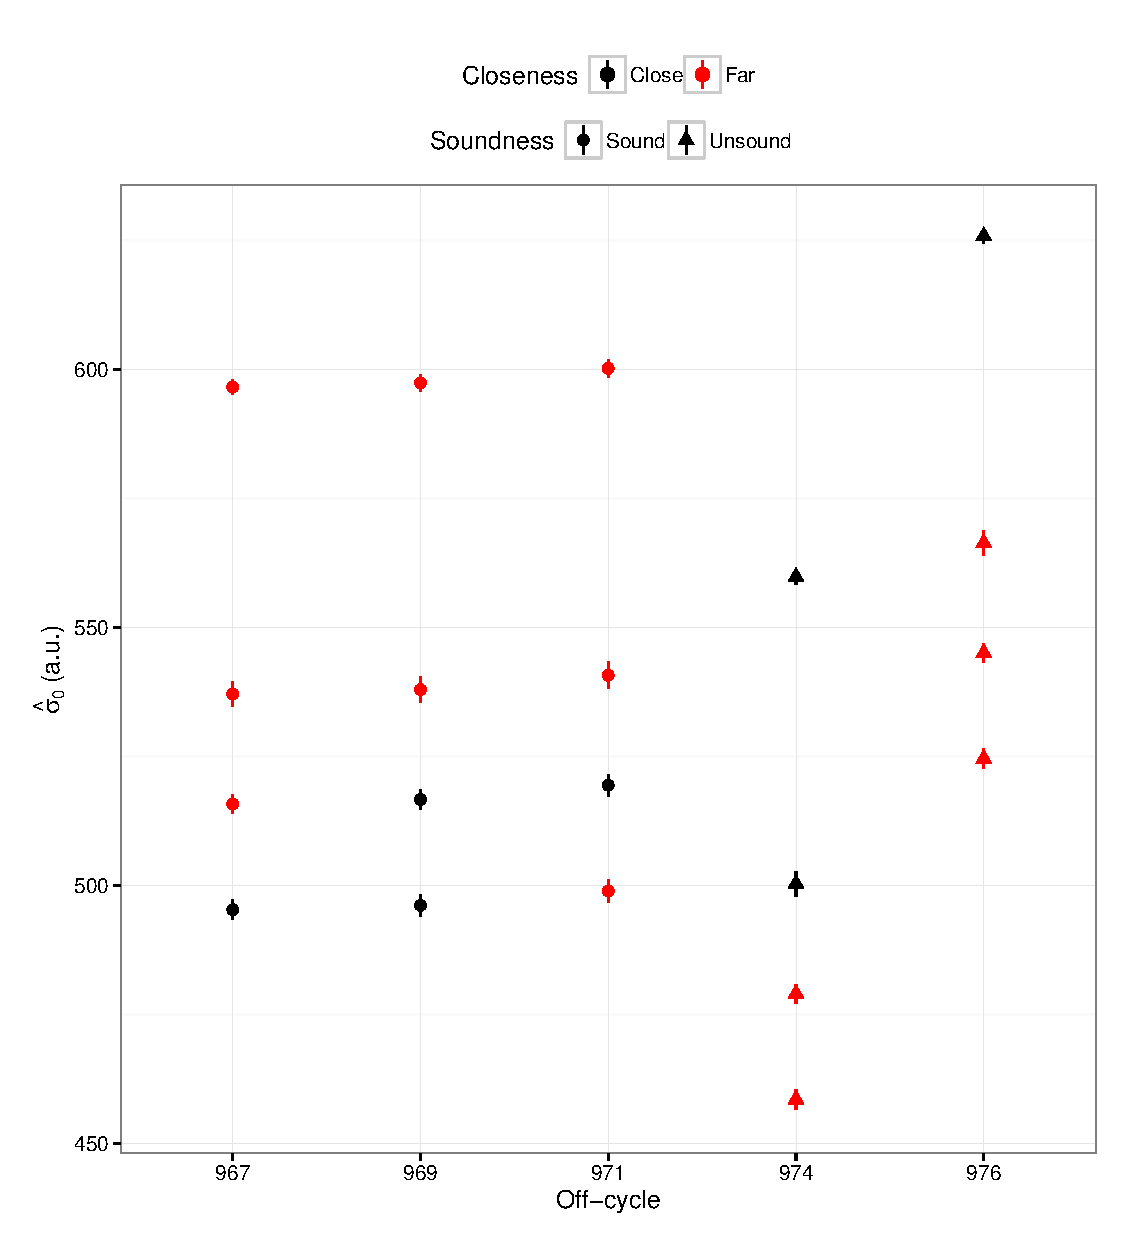
\includegraphics[scale=\scl]{img/Cross-Section2012_all.eps}
\caption{Cross section estimates plotted against their off-cycle number.\label{fig:CS-all}}
\end{subfigure}
\begin{subfigure}{.5\textwidth}
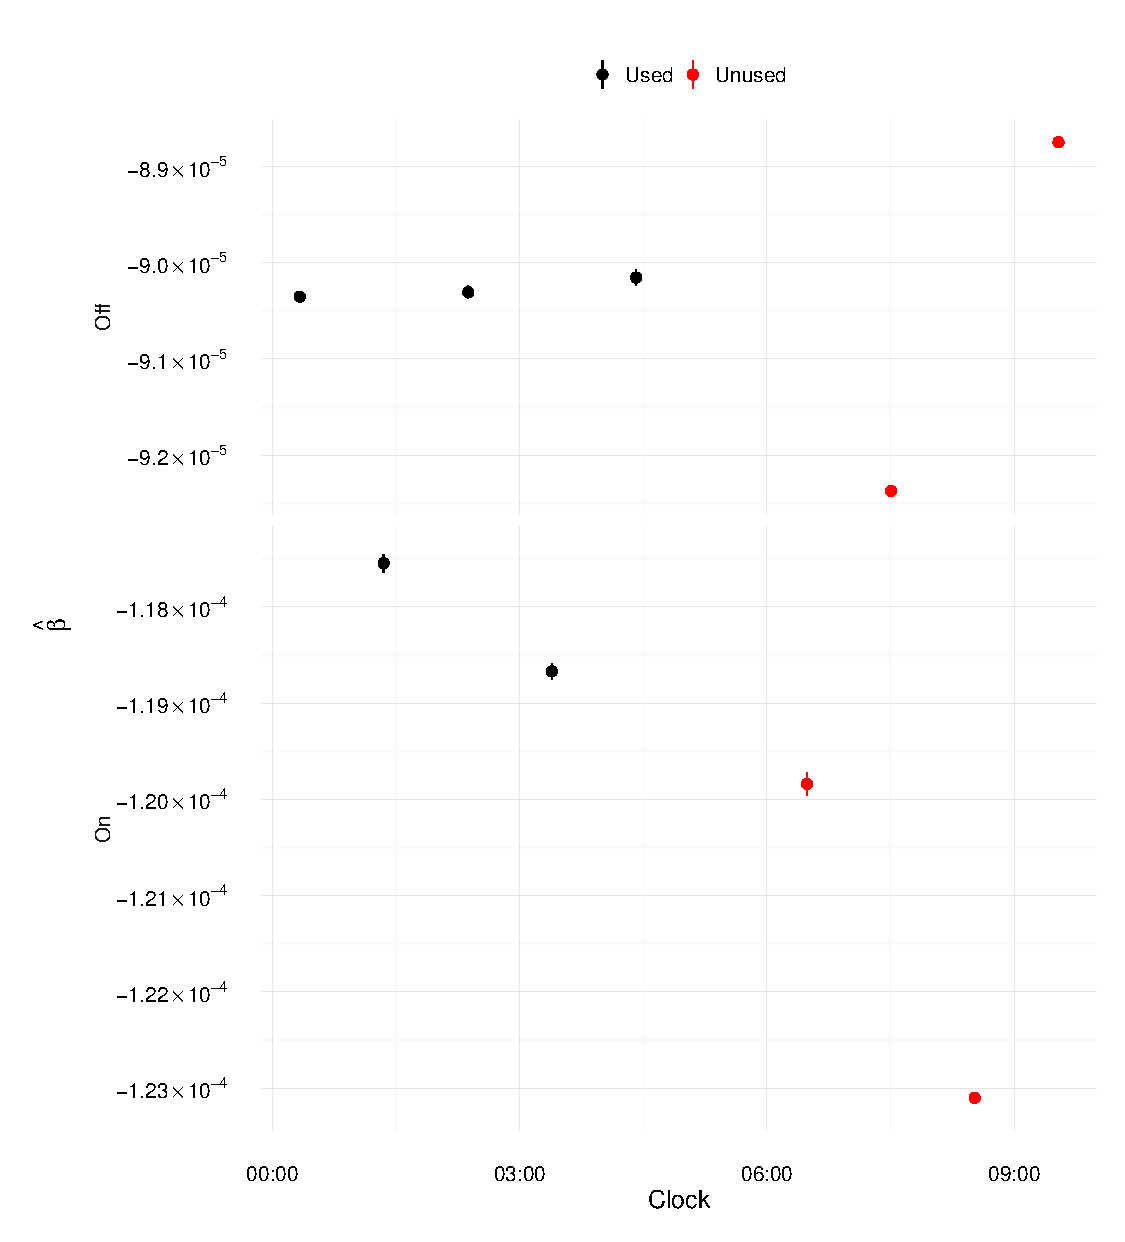
\includegraphics[scale=\scl]{img/Slopes-2012_big.eps}
\caption{Slope estimates as a function of time.\label{fig:Slopes}}
\end{subfigure}
\begin{subfigure}{.5\textwidth}
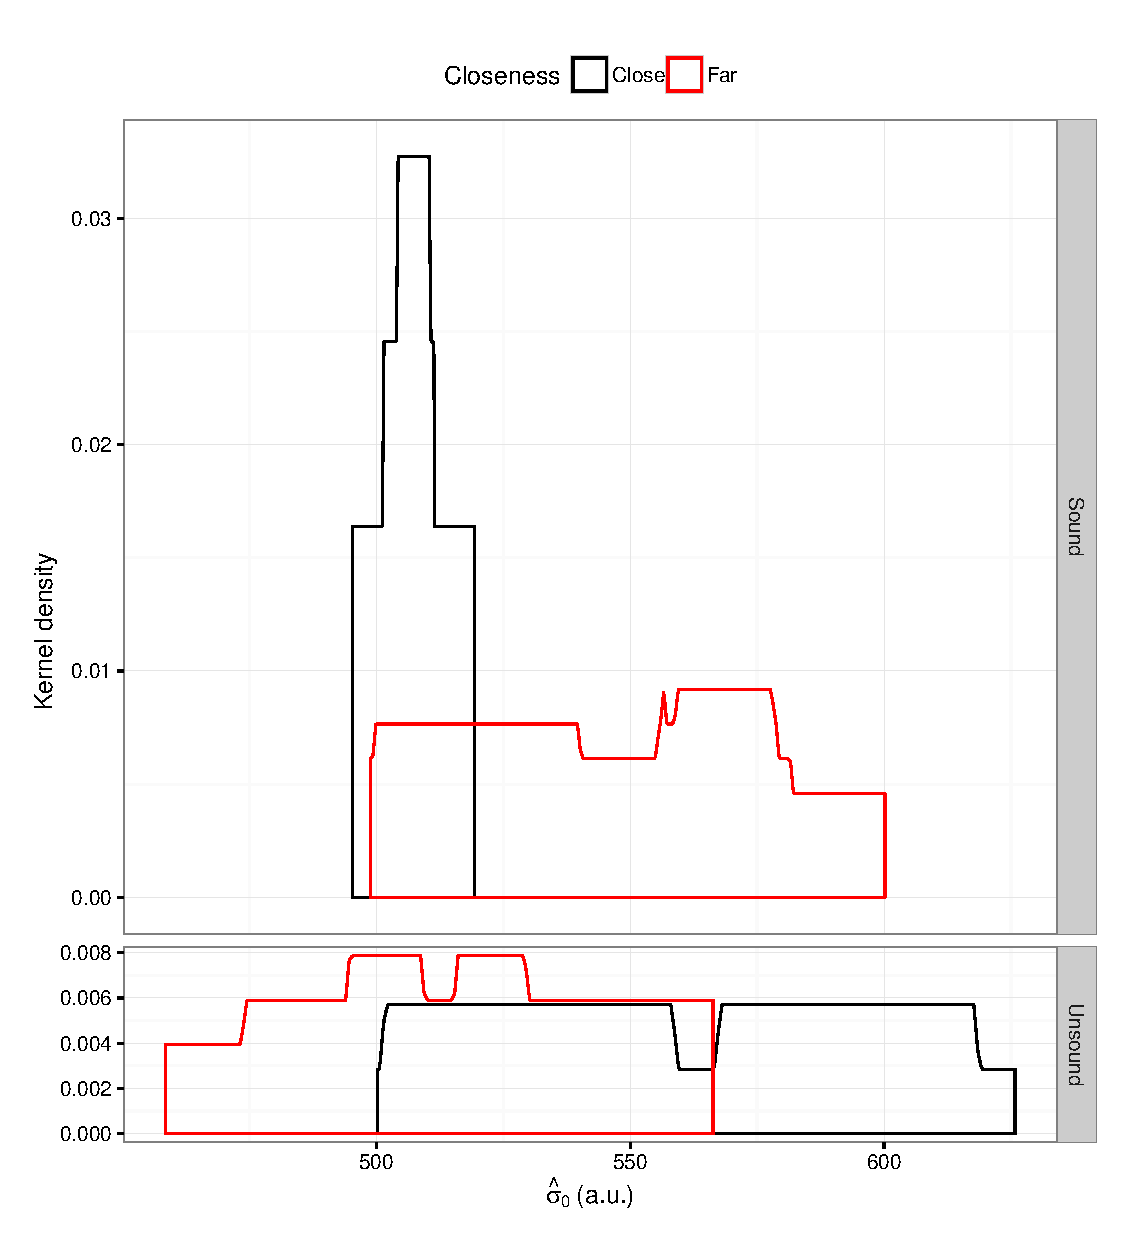
\includegraphics[scale=\scl]{img/Cross-Section2012_dens.eps}
\caption{Cross section density estimates for each category of results.\label{fig:CS-dens}}
\end{subfigure}
\caption{Results.}
\end{figure}


\begin{thebibliography}{9}
\bibitem{Conzett}
Homer E. Conzett. ``On Null Tests of Time-Reversal Invariance,'' 6. Paris, France, 1990. %\url{https://publications.lbl.gov/islandora/object/ir%3A93728/datastream/PDF/download/citation.pdf}

\bibitem{Proposal}
P.D. Eversheim, et al. ``Test of Time-Reversal Invariance in Proton-Deuteron Scattering.''
%\url{https://apps.fz-juelich.de/pax/paxwiki/images/8/8c/215-TRI_Prop_sum.pdf}

\bibitem{GaussMarkov}
D.S.G. Pollock. ``Topics in Econometrics.'' %\url{http://www.le.ac.uk/users/dsgp1/COURSES/TOPICS/gausmkov.pdf}

\end{thebibliography}

\end{document}
